%package list
\documentclass{article}
\usepackage[top=3cm, bottom=3cm, outer=3cm, inner=3cm]{geometry}
\usepackage{multicol}
\usepackage{graphicx}
\let\oldincludegraphics\includegraphics
\renewcommand{\includegraphics}[2][]{%
  \fbox{\oldincludegraphics[#1]{#2}}%
}
\setlength{\fboxsep}{0pt}    % Sin espacio entre imagen y borde
\setlength{\fboxrule}{0.8pt} 
\usepackage{url}
%\usepackage{cite}
\usepackage{hyperref}
\usepackage{array}
%\usepackage{multicol}
\newcolumntype{x}[1]{>{\centering\arraybackslash\hspace{0pt}}p{#1}}
\usepackage{natbib}
\usepackage{pdfpages}
\usepackage{multirow}
\usepackage[normalem]{ulem}
\useunder{\uline}{\ul}{}
\usepackage{svg}
\usepackage{xcolor}
\usepackage{listings}
\lstdefinestyle{ascii-tree}{
	literate={├}{|}1 {─}{--}1 {└}{+}1 
}
\lstset{basicstyle=\ttfamily,
	showstringspaces=false,
	commentstyle=\color{red},
	keywordstyle=\color{blue}
}
%\usepackage{booktabs}
\usepackage{caption}
\usepackage{subcaption}
\usepackage{float}
\usepackage{array}

\newcolumntype{M}[1]{>{\centering\arraybackslash}m{#1}}
\newcolumntype{N}{@{}m{0pt}@{}}


%%%%%%%%%%%%%%%%%%%%%%%%%%%%%%%%%%%%%%%%%%%%%%%%%%%%%%%%%%%%%%%%%%%%%%%%%%%%
%%%%%%%%%%%%%%%%%%%%%%%%%%%%%%%%%%%%%%%%%%%%%%%%%%%%%%%%%%%%%%%%%%%%%%%%%%%%
\newcommand{\itemEmail}{ }
\newcommand{\itemStudent}{
Fabiana Paola Rojas Condori
}
\newcommand{\itemCourse}{Programación Web II}
\newcommand{\itemCourseCode}{ }
\newcommand{\itemSemester}{III}
\newcommand{\itemUniversity}{Universidad Nacional de San Agustín de Arequipa}
\newcommand{\itemFaculty}{Facultad de Ingeniería de Producción y Servicios}
\newcommand{\itemDepartment}{Departamento Académico de Ingeniería de Sistemas e Informática}
\newcommand{\itemSchool}{Escuela Profesional de Ingeniería de Sistemas}
\newcommand{\itemAcademic}{2025 - A}
\newcommand{\itemOutput}{05 / 07 / 2025}
\newcommand{\itemTheme}{Angular}
%%%%%%%%%%%%%%%%%%%%%%%%%%%%%%%%%%%%%%%%%%%%%%%%%%%%%%%%%%%%%%%%%%%%%%%%%%%%
%%%%%%%%%%%%%%%%%%%%%%%%%%%%%%%%%%%%%%%%%%%%%%%%%%%%%%%%%%%%%%%%%%%%%%%%%%%%

\usepackage[english,spanish]{babel}
\usepackage[utf8]{inputenc}
\AtBeginDocument{\selectlanguage{spanish}}
\renewcommand{\figurename}{Figura}
\renewcommand{\refname}{Referencias}
\renewcommand{\tablename}{Tabla} %esto no funciona cuando se usa babel
\AtBeginDocument{%
	\renewcommand\tablename{Tabla}
}

\usepackage{fancyhdr}
\pagestyle{fancy}
\fancyhf{}
\setlength{\headheight}{30pt}
\renewcommand{\headrulewidth}{1pt}
\renewcommand{\footrulewidth}{1pt}
\fancyhead[L]{\raisebox{-0.2\height}{
\includegraphics[width=3cm]{imagenesInforme/logo_episunsa.png}}}
\fancyhead[C]{\fontsize{7}{7}\selectfont	\itemUniversity \\ \itemFaculty \\ \itemDepartment \\ \itemSchool \\ \textbf{\itemCourse}}
\fancyhead[R]{\raisebox{-0.2\height}{
\includegraphics[width=1.2cm]{imagenesInforme/logo_abet}}}
\fancyfoot[L]{Estudiante Rojas Condori Fabiana}
\fancyfoot[C]{\itemCourse}
\fancyfoot[R]{Página \thepage}

% para el codigo fuente
\usepackage{listings}
\usepackage{color, colortbl}
\definecolor{dkgreen}{rgb}{0,0.6,0}
\definecolor{gray}{rgb}{0.5,0.5,0.5}
\definecolor{mauve}{rgb}{0.58,0,0.82}
\definecolor{codebackground}{rgb}{0.95, 0.95, 0.92}
\definecolor{tablebackground}{rgb}{0.8, 0, 0}

\lstset{frame=tb,
	language=bash,
	aboveskip=3mm,
	belowskip=3mm,
	showstringspaces=false,
	columns=flexible,
	basicstyle={\small\ttfamily},
	numbers=none,
	numberstyle=\tiny\color{gray},
	keywordstyle=\color{blue},
	commentstyle=\color{dkgreen},
	stringstyle=\color{mauve},
	breaklines=true,
	breakatwhitespace=true,
	tabsize=3,
	backgroundcolor= \color{codebackground},
}

\begin{document}
	
	\vspace*{10px}
	
	\begin{center}	
		\fontsize{17}{17} \textbf{ INFORME DE ACTIVIDADES ANGULAR 1 Y 2
\itemPracticeNumber}
	\end{center}
	\centerline{\textbf{\Large Tema: \itemTheme}}
	%\vspace*{0.5cm}	
	
	\begin{flushright}
		\begin{tabular}{|M{2.5cm}|N|}
			\hline 
			\rowcolor{tablebackground}
			\color{white} \textbf{Nota}  \\
			\hline 
			\\[30pt]
			\hline 			
		\end{tabular}
	\end{flushright}	
	
	\begin{table}[H]
		\begin{tabular}{|x{4.7cm}|x{4.8cm}|x{4.8cm}|}
			\hline 
			\rowcolor{tablebackground}
			\color{white} \textbf{Estudiantes} & \color{white}\textbf{Escuela}  & \color{white}\textbf{Asignatura}   \\
			\hline 
			{\itemStudent \par \itemEmail} & \itemSchool & {\itemCourse \par Semestre: \itemSemester \par Código: \itemCourseCode}     \\
			\hline 			
		\end{tabular}
	\end{table}		
	
	\begin{table}[H]
		\begin{tabular}{|x{4.7cm}|x{4.8cm}|x{4.8cm}|}
			\hline 
			\rowcolor{tablebackground}
			\color{white}\textbf{} & \color{white}\textbf{Tema}  & \color{white}\textbf{}   \\
			\hline 
			\itemPracticeNumber & \itemTheme & -   \\
			\hline 
		\end{tabular}
	\end{table}
	
	\begin{table}[H]
		\begin{tabular}{|x{4.7cm}|x{4.8cm}|x{4.8cm}|}
			\hline 
			\rowcolor{tablebackground}
			\color{white}\textbf{Semestre académico} & \color{white}\textbf{Fecha de inicio}  & \color{white}\textbf{Fecha de entrega}   \\
			\hline 
			\itemAcademic & \itemInput &  \itemOutput  \\
			\hline 
		\end{tabular}
	\end{table}
	
	\section{Presentación de la Tarea}
	\begin{itemize}		
		\item Volver a implementar las clases teóricas en un proyecto en github realizando commits de cada avance.  Compartirlo con el profesor sacando un pantallazo de los commits y agregandolo al informe.
		
		
	\end{itemize}
	
	\section{Equipos, materiales y temas utilizados }
	\begin{itemize}
		\item \textbf{Visual Studio Code}: Editor de código fuente utilizado como entorno principal de desarrollo.
  \item \textbf{Angular CLI (versión 20)}: Herramienta de línea de comandos para crear componentes, servicios y gestionar el proyecto.
  \item \textbf{Node.js y npm}: Para ejecutar y administrar dependencias del proyecto.
  \item \textbf{Git}: Sistema de control de versiones para registrar los cambios realizados en cada etapa del proyecto.
  \item \textbf{Cuenta en GitHub}: Utilizada para almacenar el repositorio del proyecto con una cuenta institucional.
  \item \textbf{Framework Angular}: Utilizado para desarrollar la aplicación con arquitectura basada en componentes. Se aplicaron conceptos como data binding, servicios, formularios, rutas y uso de componentes standalone.
  \item \textbf{Sistema operativo}: Ubuntu (vía WSL) para ejecutar los comandos en la terminal de forma fluida.
  \item \textbf{LaTeX}: Para la redacción y estructura del informe final técnico.
		
	\end{itemize}
	
	\section{URL de Repositorio Github}
	\begin{itemize}
		\item URL del Repositorio GitHub general.
		\item \url{https://github.com/FabianaRojasCondori/PW2-TEORIA.git}
        
		\item URL para Angular 1 y2  en el Repositorio GitHub.
		\item \url{https://github.com/FabianaRojasCondori/PW2-TEORIA/tree/main/proyectoAngular/my-dream-app}
        \item URL para el proyecto visto en la nube desde vercel
		\item \url{https://angular-ekpk.vercel.app/}
	\end{itemize}	
	\section{Estructura del proyecto}
	
	\begin{itemize}	
		\item Contenido presente en my-dream-app
	\end{itemize}
	
	\begin{lstlisting}[style=ascii-tree]
		my-dream-app/
           ├── angular.json
           ├── dist
           ├── node_modules
           ├── package-lock.json
           ├── package.json
           ├── public
           ├── src
           ├── tsconfig.app.json
           ├── tsconfig.json
           └── tsconfig.spec.json
		
	\end{lstlisting}

\begin{itemize}	
		\item Carpeta src
	\end{itemize}

\begin{lstlisting}[style=ascii-tree]
.
├── app
│   ├── Post.ts
│   ├── about
│   │   ├── about.css
│   │   ├── about.html
│   │   ├── about.spec.ts
│   │   └── about.ts
│   ├── app.component.css
│   ├── app.component.html
│   ├── app.component.ts
│   ├── app.config.ts
│   ├── app.css
│   ├── app.html
│   ├── app.routes.ts
│   ├── app.spec.ts
│   ├── app.ts
│   ├── data.service.ts
│   ├── data.spec.ts
│   ├── data.ts
│   ├── hello-world
│   │   ├── hello-world.css
│   │   ├── hello-world.html
│   │   ├── hello-world.spec.ts
│   │   └── hello-world.ts
│   └── user
│       ├── user.css
│       ├── user.html
│       ├── user.spec.ts
│       └── user.ts
├── index.html
├── main.ts
└── styles.css
\end{lstlisting}

    

        \section{Commits realizados}

        A continuación se muestran los commit más relevantes que fueron realizados en cada rama de los integrantes. 

	
        
    \begin{lstlisting}
    Commit1: angular1 - Diapositiva 11: Se realizaron las instalaciones y el primer desarrollo en angular}
\end{lstlisting}
En esta primera parte del desarrollo se crearon los componentes requeridos y se empezó con el desarrollo del código indicado en las diapositivas. La visualización de dichos cambios se muestra a continuación. 

\begin{center}
    \makebox[0pt]{Ejecución}
\end{center}

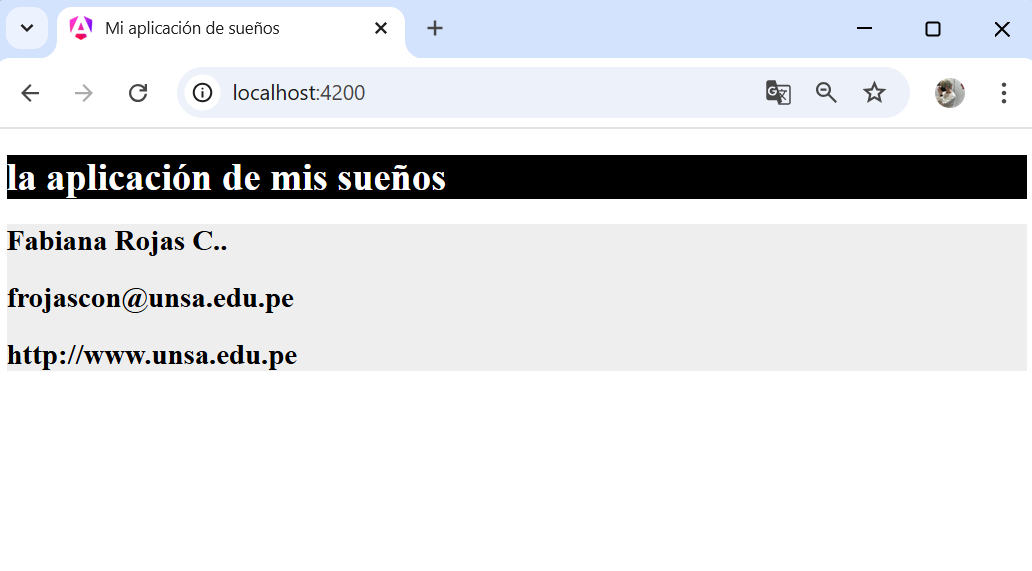
\includegraphics[width=1\textwidth,keepaspectratio]{imagenesInforme/P1.png}
		%\includesvg{imagenesInforme/P1.png}
		%\label{img:mot2}
		%\caption{Product backlog.}
	\end{figure}

     \begin{lstlisting}
    Commit 2: Angular1 - Diapositivas 13,14: Se agrego un constructor en app.component.ts y se usaron For e Ifs para mostrar los hobbies
\end{lstlisting}
Durante esta etapa, se implementó una sección dinámica para mostrar los hobbies del usuario utilizando Angular. Se incorporaron directivas estructurales como *ngIf y *ngFor, controladas por un método showhobbies() y una propiedad hobbies definida en el componente. Además, se aplicaron estilos personalizados mediante clases CSS (.black, .ash, .component2) para mejorar la presentación visual del contenido, logrando una interfaz clara y segmentada. Estos cambios permitieron integrar datos personales, navegación fluida y componentes visuales.

\begin{center}
    \makebox[0pt]{Ejecución}
\end{center}

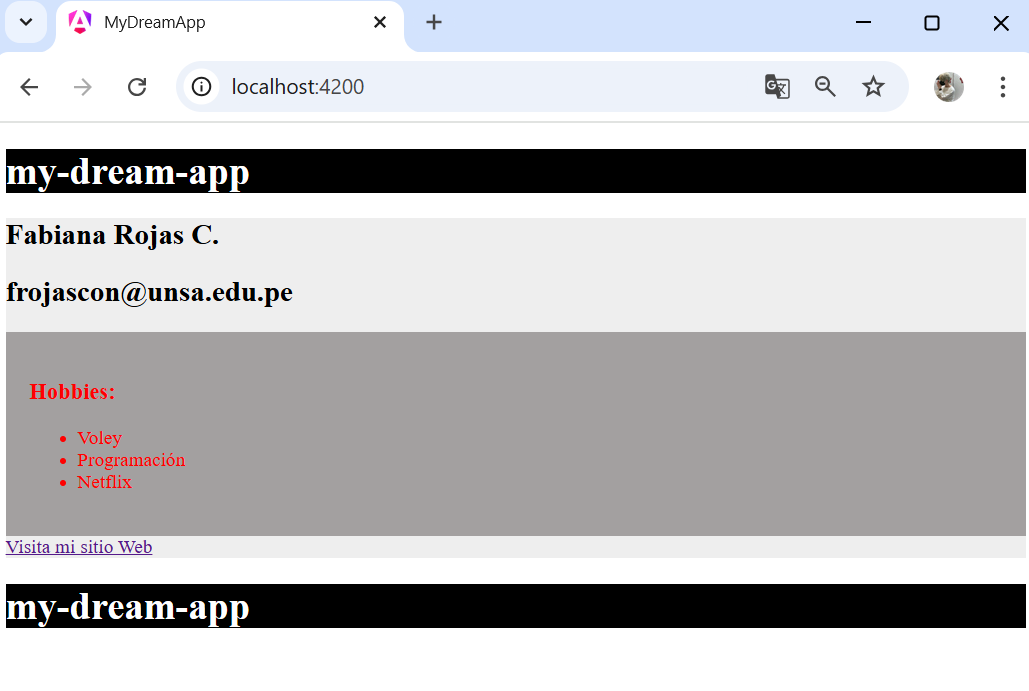
\includegraphics[width=1\textwidth,keepaspectratio]{imagenesInforme/P2.png}
		%\includesvg{imagenesInforme/P1.png}
		%\label{img:mot2}
		%\caption{Product backlog.}
	\end{figure}
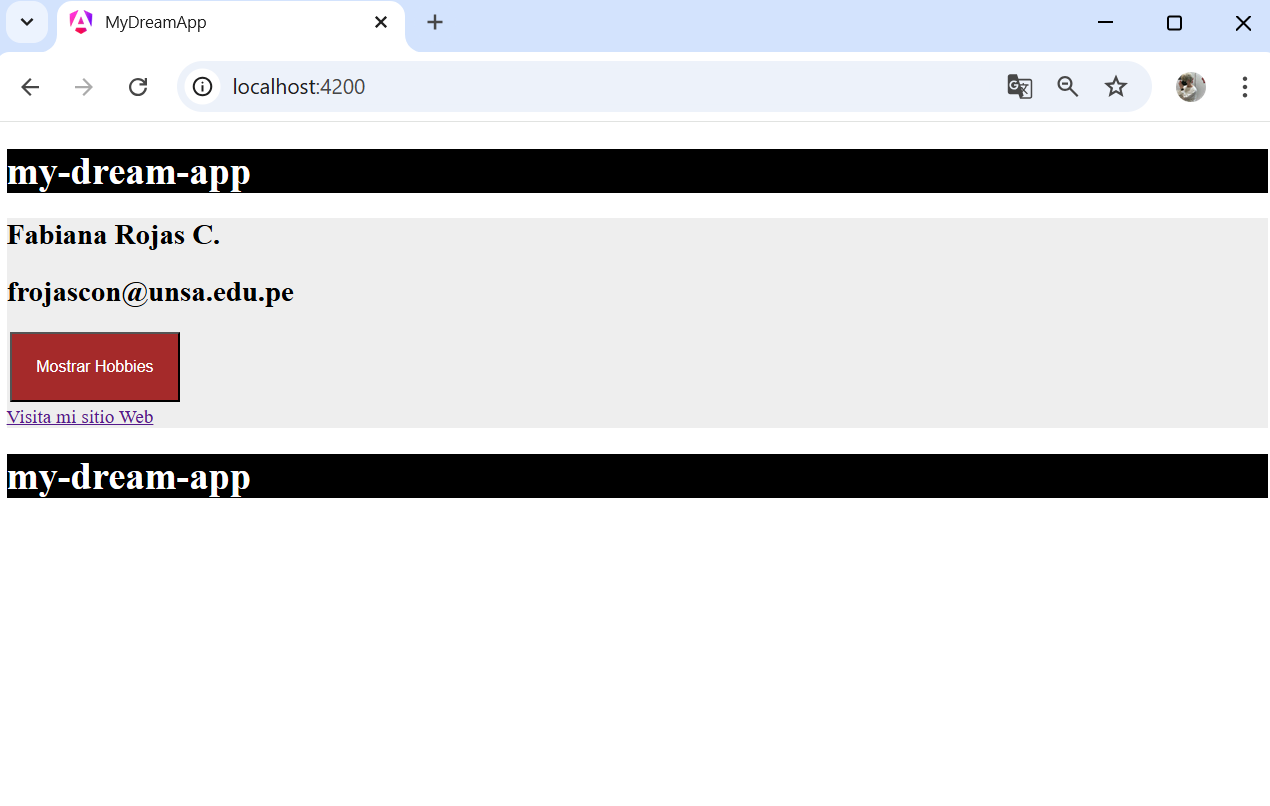
\includegraphics[width=1\textwidth,keepaspectratio]{imagenesInforme/P3.png}
		%\includesvg{imagenesInforme/P1.png}
		%\label{img:mot2}
		%\caption{Product backlog.}
	\end{figure}
    
\begin{lstlisting}
    Commit 3: "Angular1 - Diapositiva 16: Se agrega un botón para mostrar Hobbies."

\end{lstlisting}
se añadió interactividad a la sección de hobbies mediante un botón con clase personalizada .btn, el cual permite mostrar u ocultar dinámicamente la lista de actividades favoritas del usuario. Para lograrlo, se implementó en app.component.ts la propiedad booleana showHobbies y el método toggleHobbies(), vinculados al botón mediante un evento (click). Además, se aplicaron estilos visuales distintivos a través de clases CSS (.component2, .btn) que mejoran la presentación visual y refuerzan la experiencia de usuario en la interfaz Angular.

\begin{center}
    \makebox[0pt]{Ejecución}
\end{center}

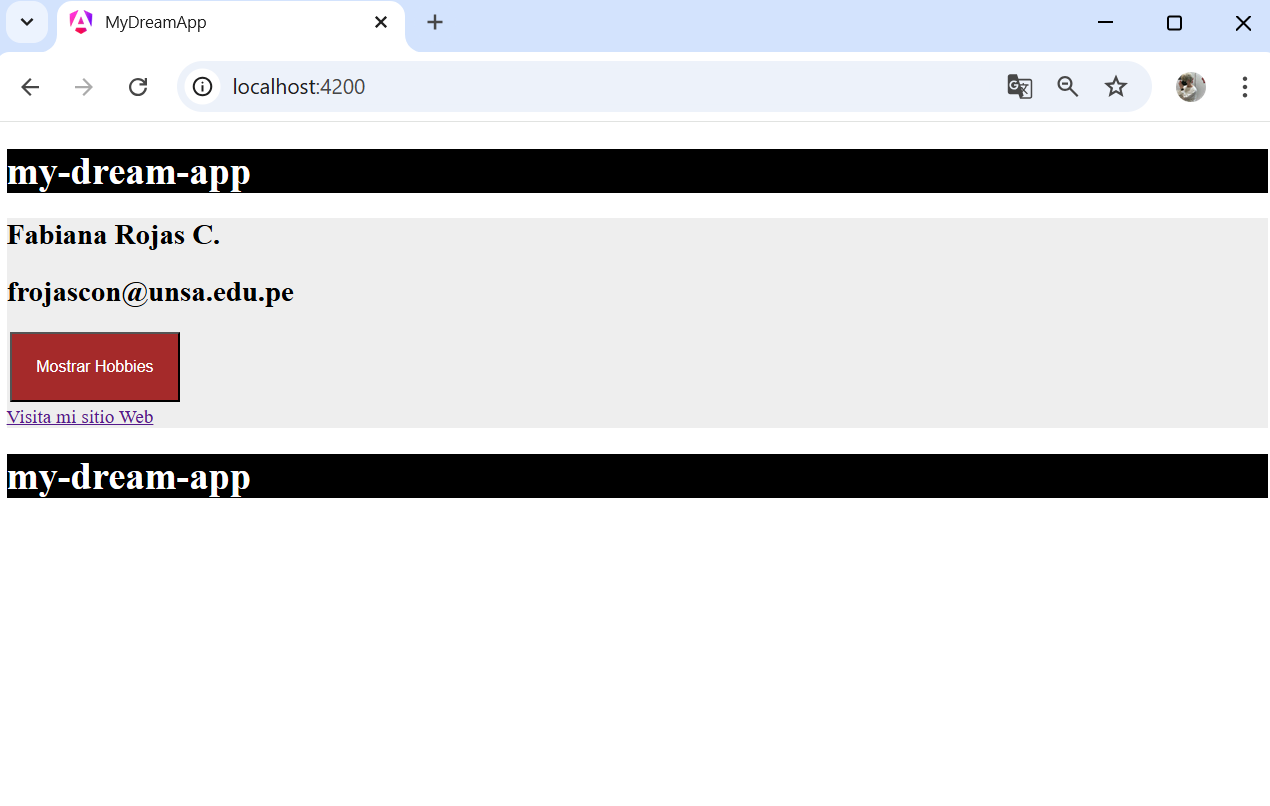
\includegraphics[width=1\textwidth,keepaspectratio]{imagenesInforme/P5.png}
		%\includesvg{imagenesInforme/P1.png}
		%\label{img:mot2}
		%\caption{Product backlog.}
	\end{figure}

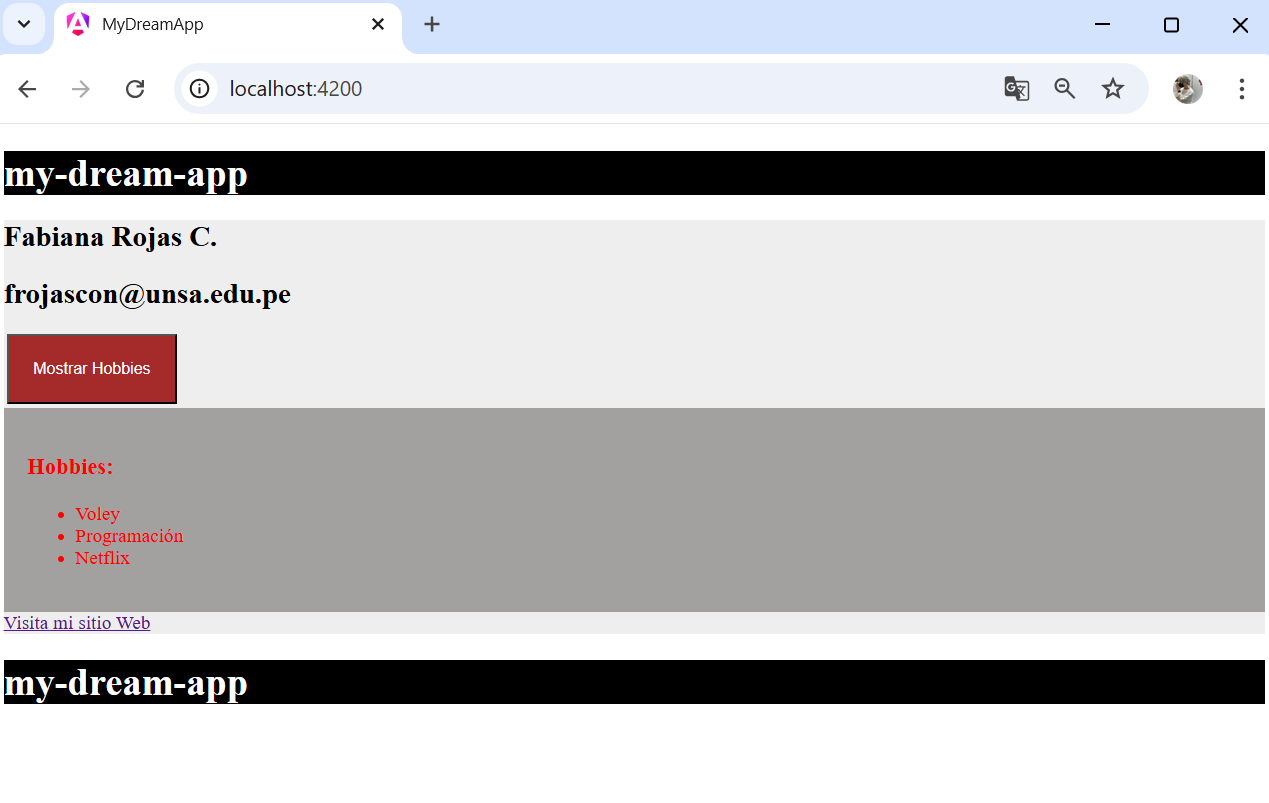
\includegraphics[width=1\textwidth,keepaspectratio]{imagenesInforme/P4.png}
		%\includesvg{imagenesInforme/P1.png}
		%\label{img:mot2}
		%\caption{Product backlog.}
	\end{figure}

\begin{lstlisting}
    Commit 4: "Angular1 - Diapositiva 17: Se agrega un form para poder añadir más Hobbies."

\end{lstlisting}
se incorporó un formulario dentro de la sección de hobbies que permite al usuario añadir nuevas actividades de forma dinámica. Para lograr esta funcionalidad, se implementó el método newHobby() en el componente principal, el cual se activa al enviar el formulario y agrega el valor ingresado al arreglo hobbies. Además, se actualizó el HTML utilizando referencias locales y la directiva (submit) para captar los datos introducidos. 

\begin{center}
    \makebox[0pt]{Ejecución}
\end{center}
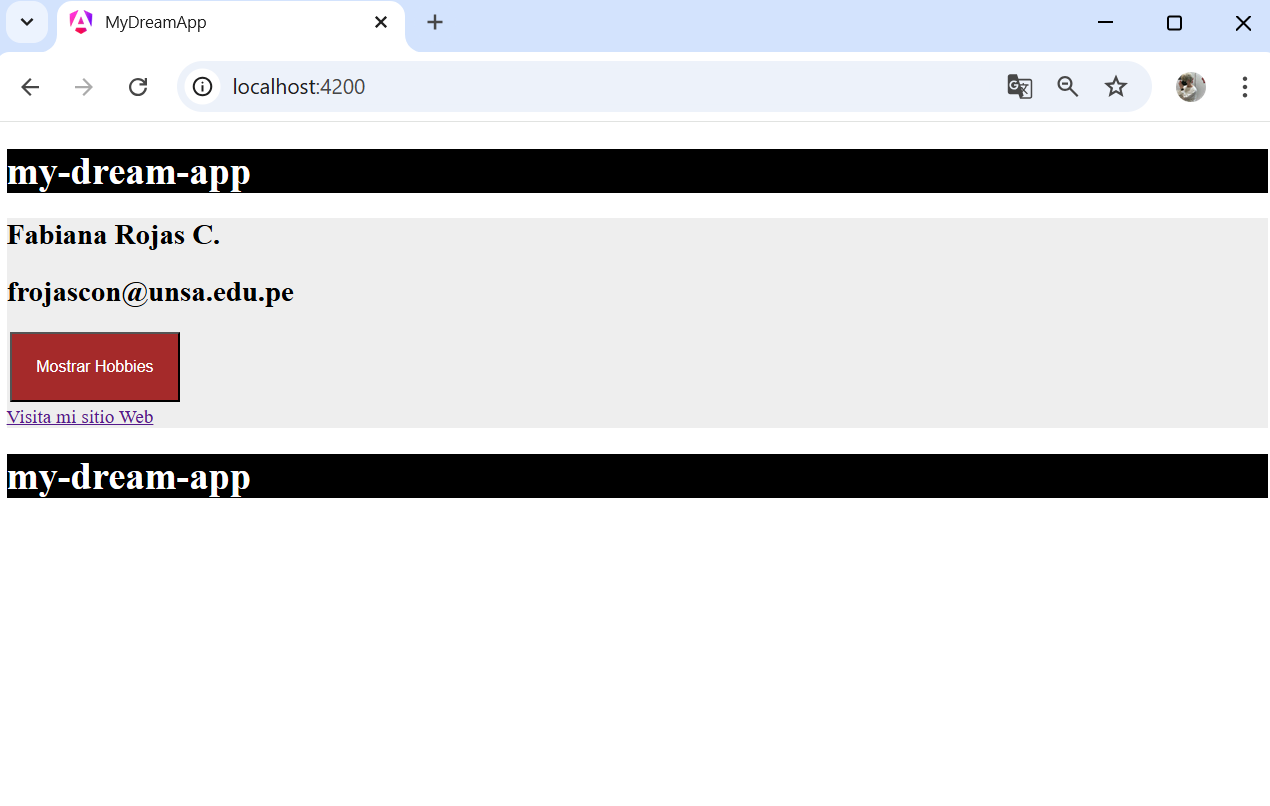
\includegraphics[width=1\textwidth,keepaspectratio]{imagenesInforme/P6.png}
		%\includesvg{imagenesInforme/P1.png}
		%\label{img:mot2}
		%\caption{Product backlog.}
	\end{figure}
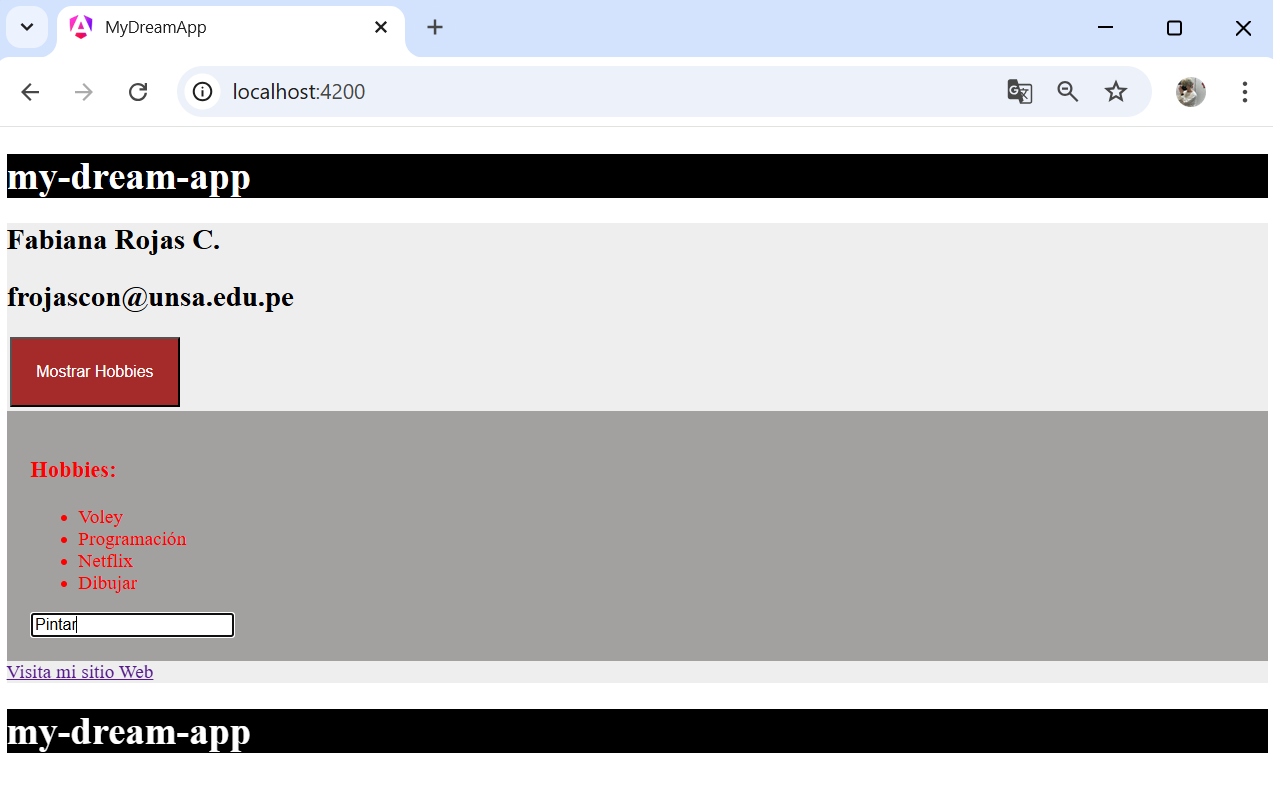
\includegraphics[width=1\textwidth,keepaspectratio]{imagenesInforme/P7.png}
		%\includesvg{imagenesInforme/P1.png}
		%\label{img:mot2}
		%\caption{Product backlog.}
	\end{figure}
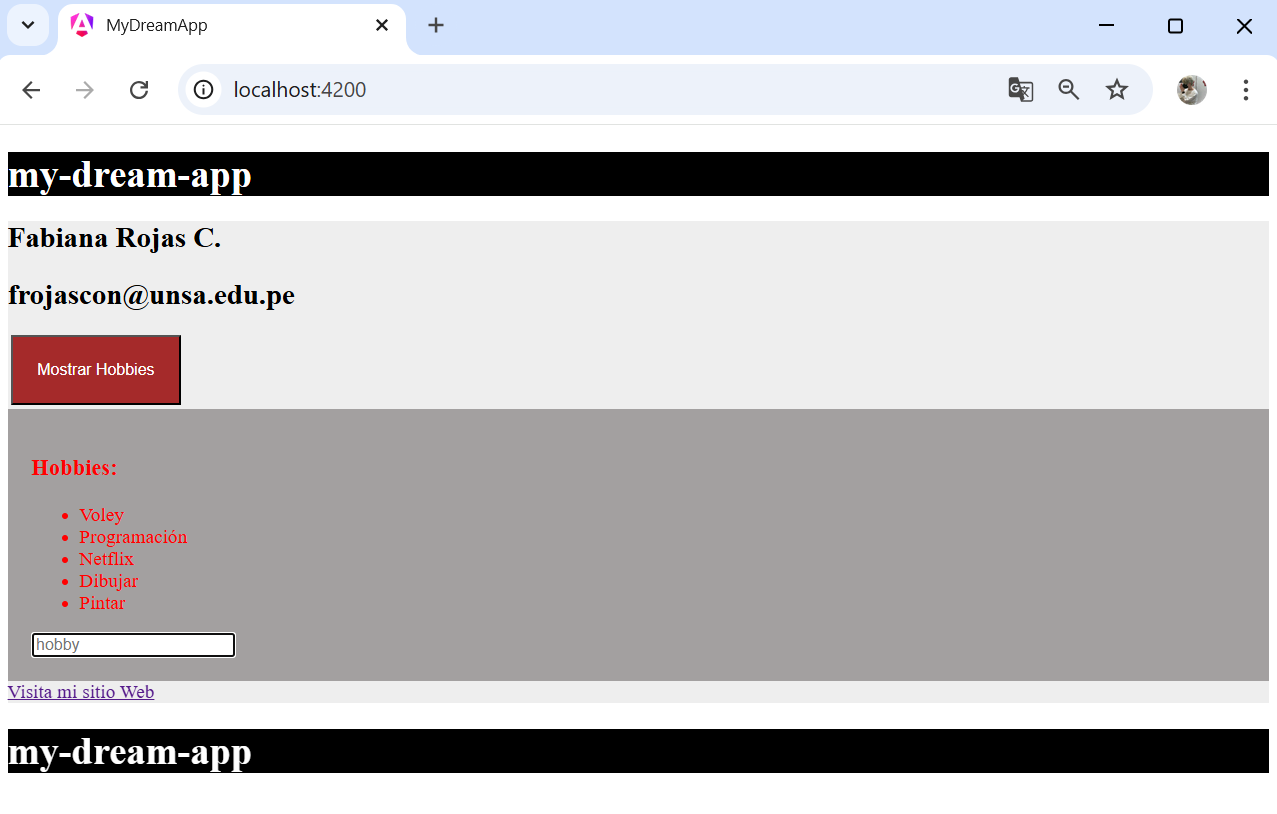
\includegraphics[width=1\textwidth,keepaspectratio]{imagenesInforme/P8.png}
		%\includesvg{imagenesInforme/P1.png}
		%\label{img:mot2}
		%\caption{Product backlog.}
	\end{figure}
\begin{lstlisting}
     Commit 5: "Angular1 - Diapositiva 20: Se genero el componente hello-world."
\end{lstlisting}
 se generó el componente hello-world como parte del proceso de modularización de la aplicación. Este nuevo componente fue creado con una estructura standalone y se integró al AppComponent tanto en el arreglo de imports como en la plantilla HTML mediante el selector <app-hello-world>. Además, se añadieron sus archivos asociados (.ts, .html, .css, y .spec.ts) para asegurar su correcto funcionamiento, visualización y testeo.
\begin{center}
    \makebox[0pt]{Ejecución}
\end{center}
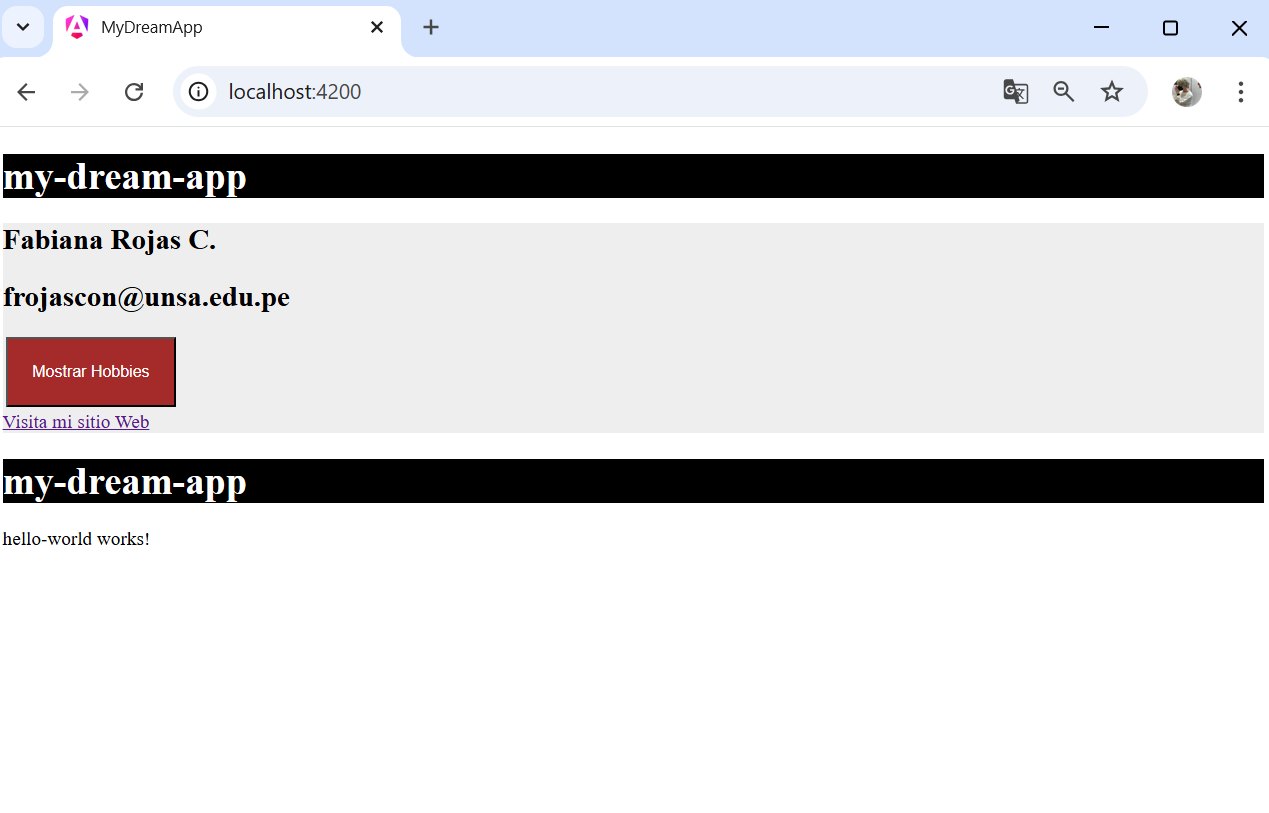
\includegraphics[width=1\textwidth,keepaspectratio]{imagenesInforme/P9.png}
		%\includesvg{imagenesInforme/P1.png}
		%\label{img:mot2}
		%\caption{Product backlog.}
	\end{figure}
\begin{lstlisting}
     Commit 6:  "Angular1 - Diapositiva 22: Se pasaron datos al componente user y se crearon 'ryan, joe, cameron, john' segun indicaciones."
\end{lstlisting}
 se incorporó el componente user al proyecto con el objetivo de representar a cada usuario de manera individual y reutilizable. Se definió una propiedad users en el componente principal (AppComponent) con los nombres 'ryan', 'joe', 'cameron' y 'john', y se utilizó *ngFor para recorrer ese arreglo en la plantilla. A través de @Input(), se pasó dinámicamente cada nombre al componente user, el cual se encargó de renderizarlos dentro de su propia vista (user.html).
\begin{center}
    \makebox[0pt]{Ejecución}
\end{center}
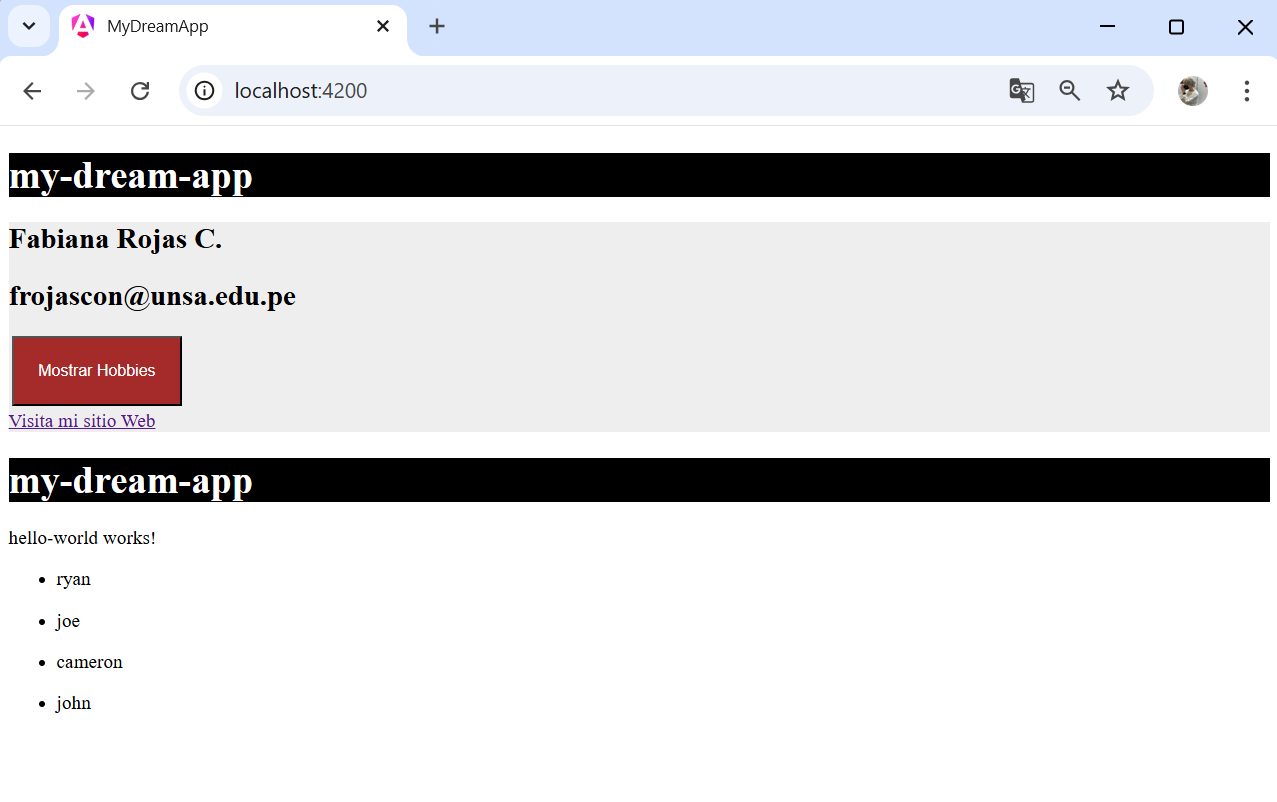
\includegraphics[width=1\textwidth,keepaspectratio]{imagenesInforme/P10.png}
		%\includesvg{imagenesInforme/P1.png}
		%\label{img:mot2}
		%\caption{Product backlog.}
	\end{figure}

\begin{lstlisting}
Commit 7: "Angular1 - Diapositiva 23: Se agregan botones de alerta a la aplicacion para que cada usuario tenga un boton que diga un mensaje('Hazme click solo a mi)."
\end{lstlisting}
se mejoró la interacción en el componente user incorporando un botón personalizado para cada elemento de la lista de usuarios. Mediante la función sayHello(nameUser), se activó una alerta que muestra un mensaje específico con el nombre del usuario al hacer clic en su botón. Esta funcionalidad fue implementada utilizando @Input() para recibir el dato del nombre y una función de alerta vinculada al evento (click).
\begin{center}
    \makebox[0pt]{Ejecución}
\end{center}
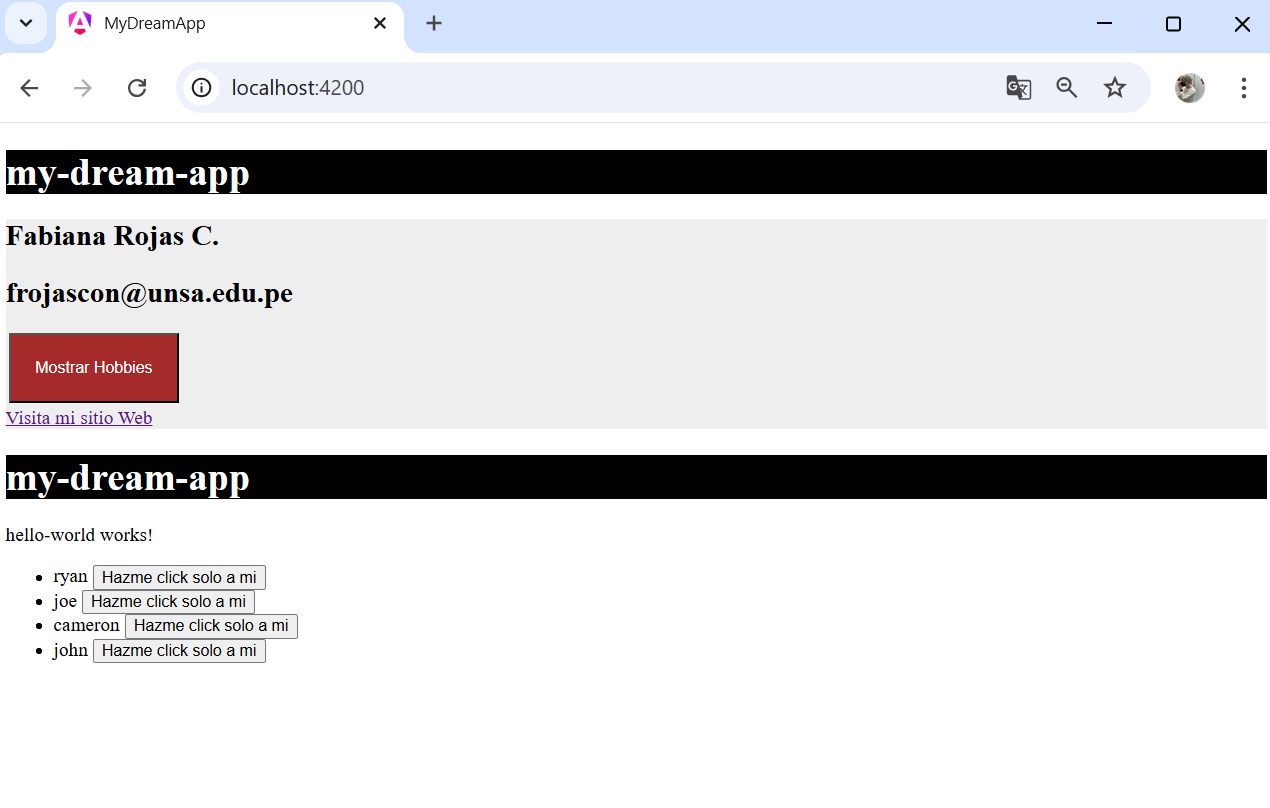
\includegraphics[width=1\textwidth,keepaspectratio]{imagenesInforme/P11.png}
		%\includesvg{imagenesInforme/P1.png}
		%\label{img:mot2}
		%\caption{Product backlog.}
	\end{figure}
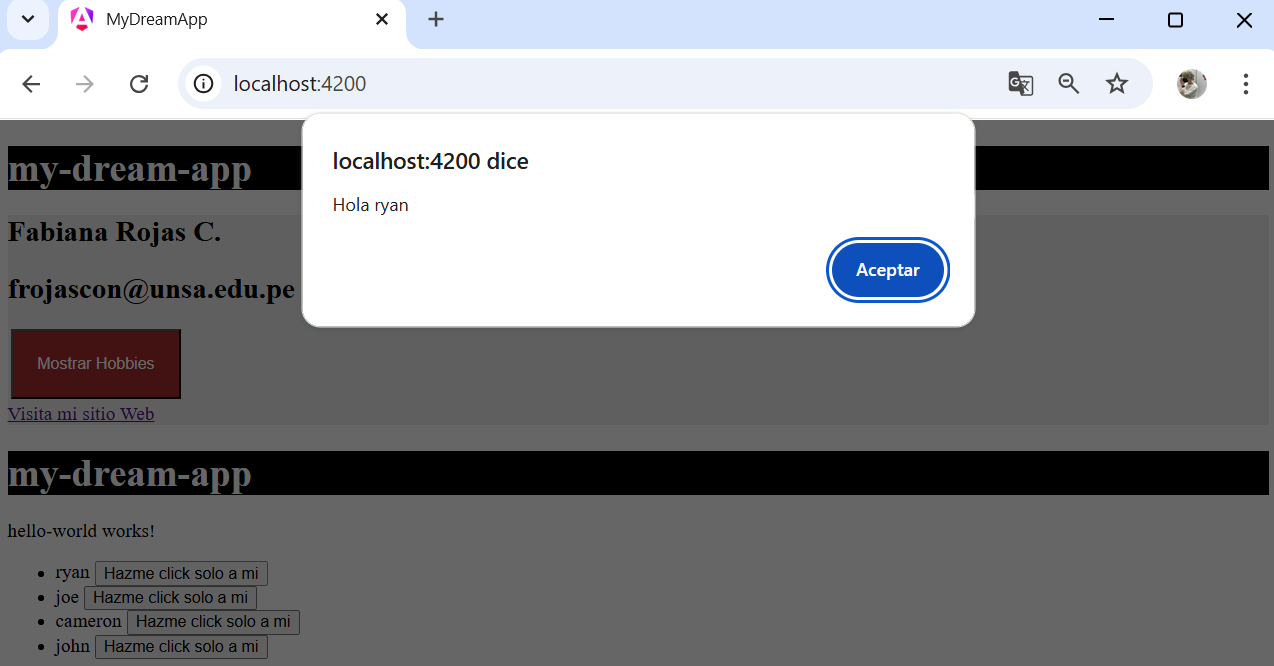
\includegraphics[width=1\textwidth,keepaspectratio]{imagenesInforme/P12.png}
		%\includesvg{imagenesInforme/P1.png}
		%\label{img:mot2}
		%\caption{Product backlog.}
	\end{figure}
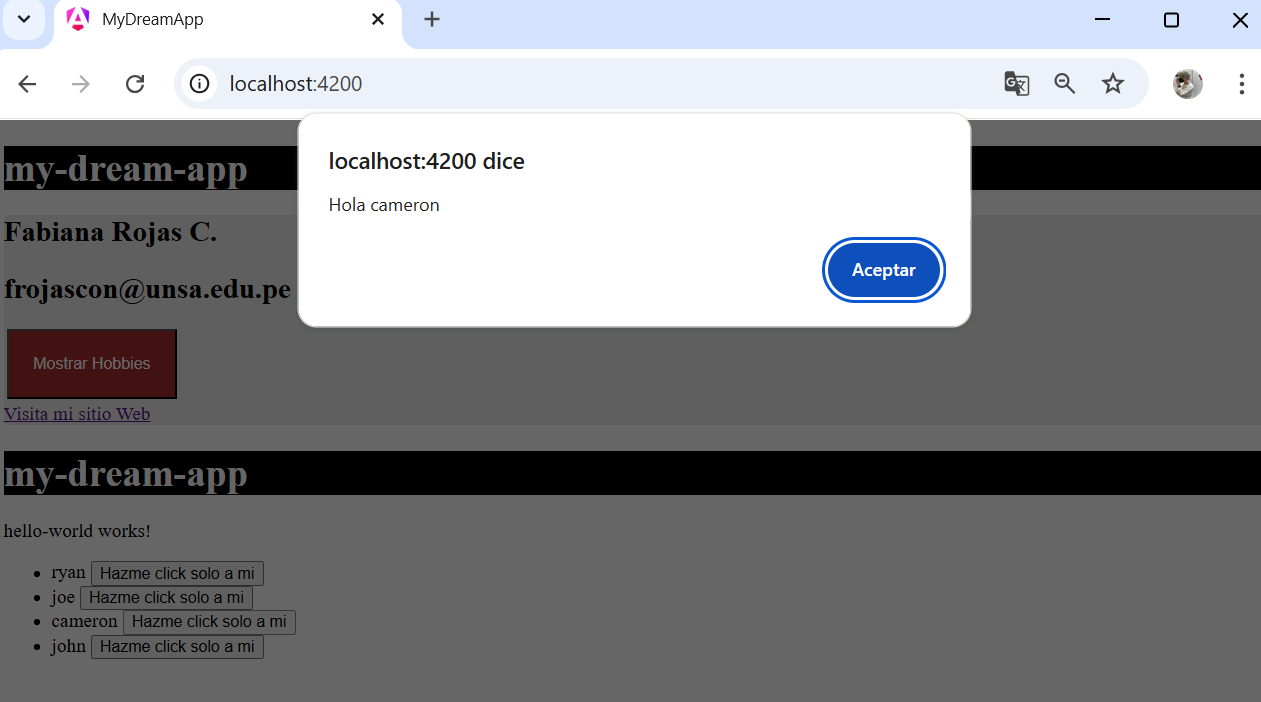
\includegraphics[width=1\textwidth,keepaspectratio]{imagenesInforme/P13.png}
		%\includesvg{imagenesInforme/P1.png}
		%\label{img:mot2}
		%\caption{Product backlog.}
	\end{figure}
\begin{lstlisting}
Commit 8: "Angular1 - Diapositiva 24: Se agregan botones que borran elementos de una lista (usuarios)."
\end{lstlisting}
En el Commit 8, correspondiente a la Diapositiva 24, se añadió la funcionalidad para eliminar usuarios individualmente desde la vista principal del componente. Para lograrlo, se implementó el método deleteUser(user) dentro de AppComponent, el cual recorre el arreglo users y remueve el elemento seleccionado. Esta lógica fue integrada al HTML mediante un botón por cada usuario, enlazado con (click)="deleteUser(user)", lo que permitió una experiencia más interactiva y dinámica, fortaleciendo el manejo de eventos y manipulación de listas en Angular.
\begin{center}
    \makebox[0pt]{Ejecución}
\end{center}
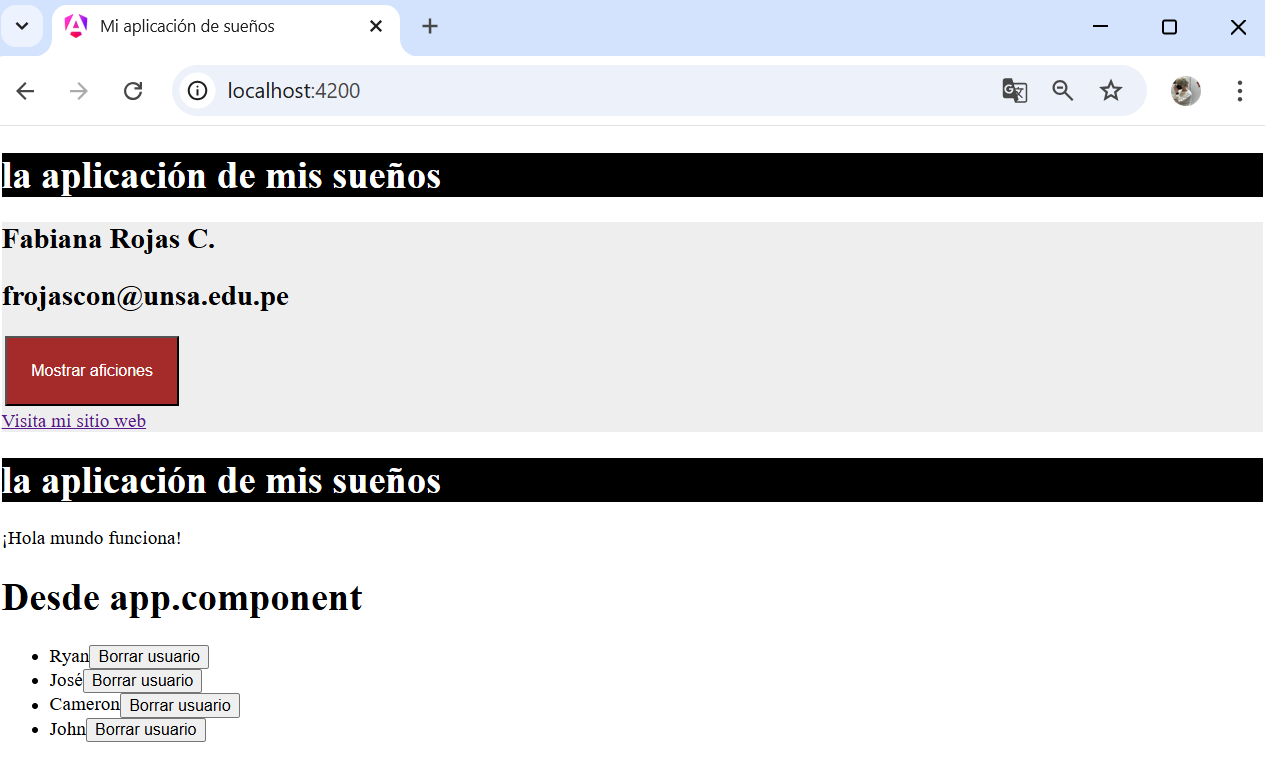
\includegraphics[width=1\textwidth,keepaspectratio]{imagenesInforme/P14.png}
		%\includesvg{imagenesInforme/P1.png}
		%\label{img:mot2}
		%\caption{Product backlog.}
	\end{figure}
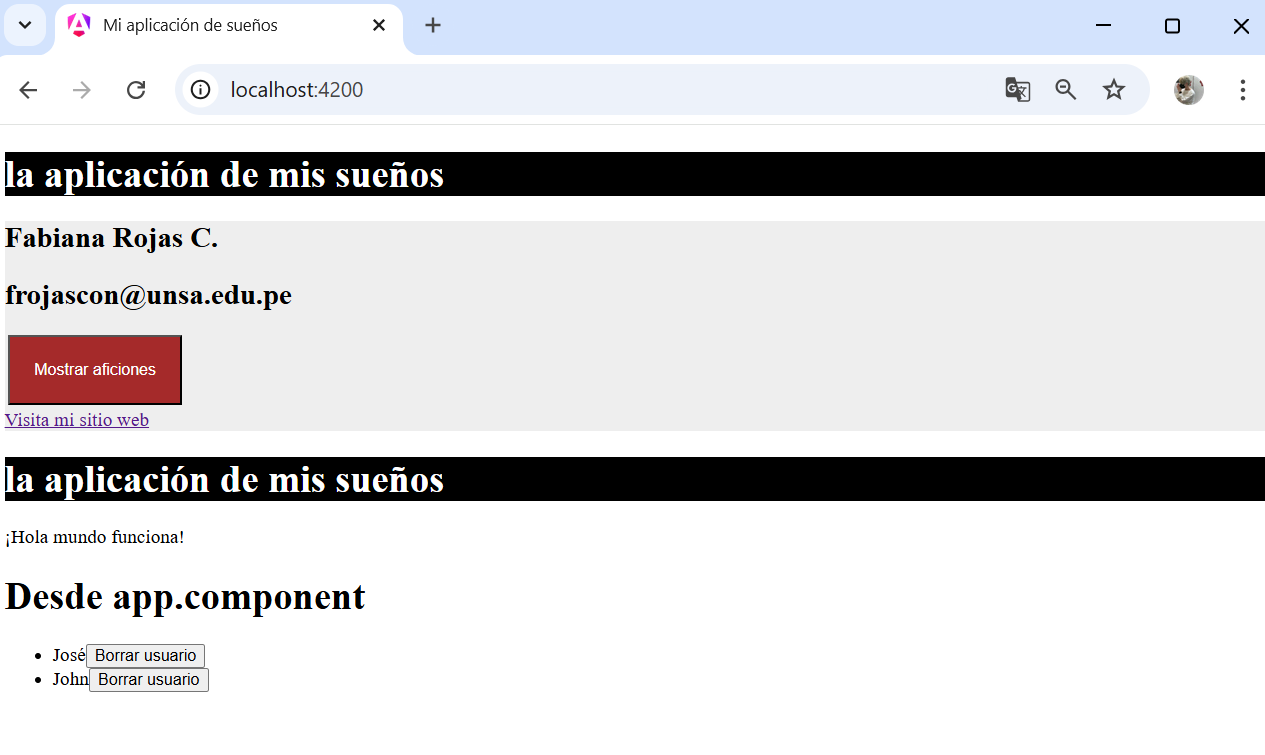
\includegraphics[width=1\textwidth,keepaspectratio]{imagenesInforme/P15.png}
		%\includesvg{imagenesInforme/P1.png}
		%\label{img:mot2}
		%\caption{Product backlog.}
	\end{figure}

\begin{lstlisting}
Commit 9:  "Angular1 - Diapositiva 26: Pasando referencias del Formulario - Ahora se puede agregar y eliminar usuarios."
\end{lstlisting}
\begin{center}
    \makebox[0pt]{Ejecución}
\end{center}
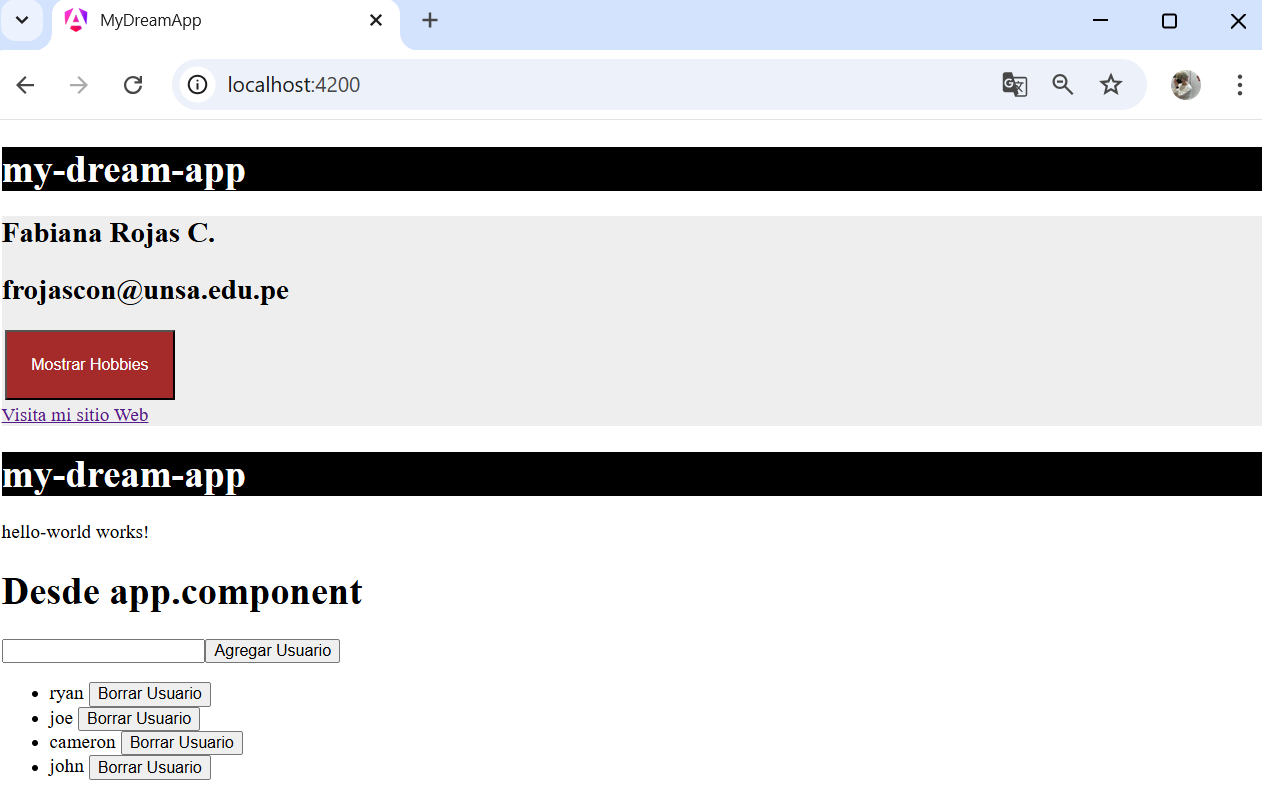
\includegraphics[width=1\textwidth,keepaspectratio]{imagenesInforme/P16.png}
		%\includesvg{imagenesInforme/P1.png}
		%\label{img:mot2}
		%\caption{Product backlog.}
	\end{figure}
\begin{lstlisting}
Commit 10:  "Angular1: Se muestra boton de alerta y se puede agregar y eliminar usuarios"
\end{lstlisting}
se mejoró la funcionalidad de gestión de usuarios mediante el uso de referencias locales en formularios. Se implementó un formulario que permite añadir usuarios a la lista utilizando #newUser como referencia directa al input, lo cual se vinculó al método addUser() mediante la directiva (submit). Además, se mantuvo la posibilidad de eliminar usuarios con el botón asociado a la función deleteUser(). 
\begin{center}
    \makebox[0pt]{Ejecución}
\end{center}
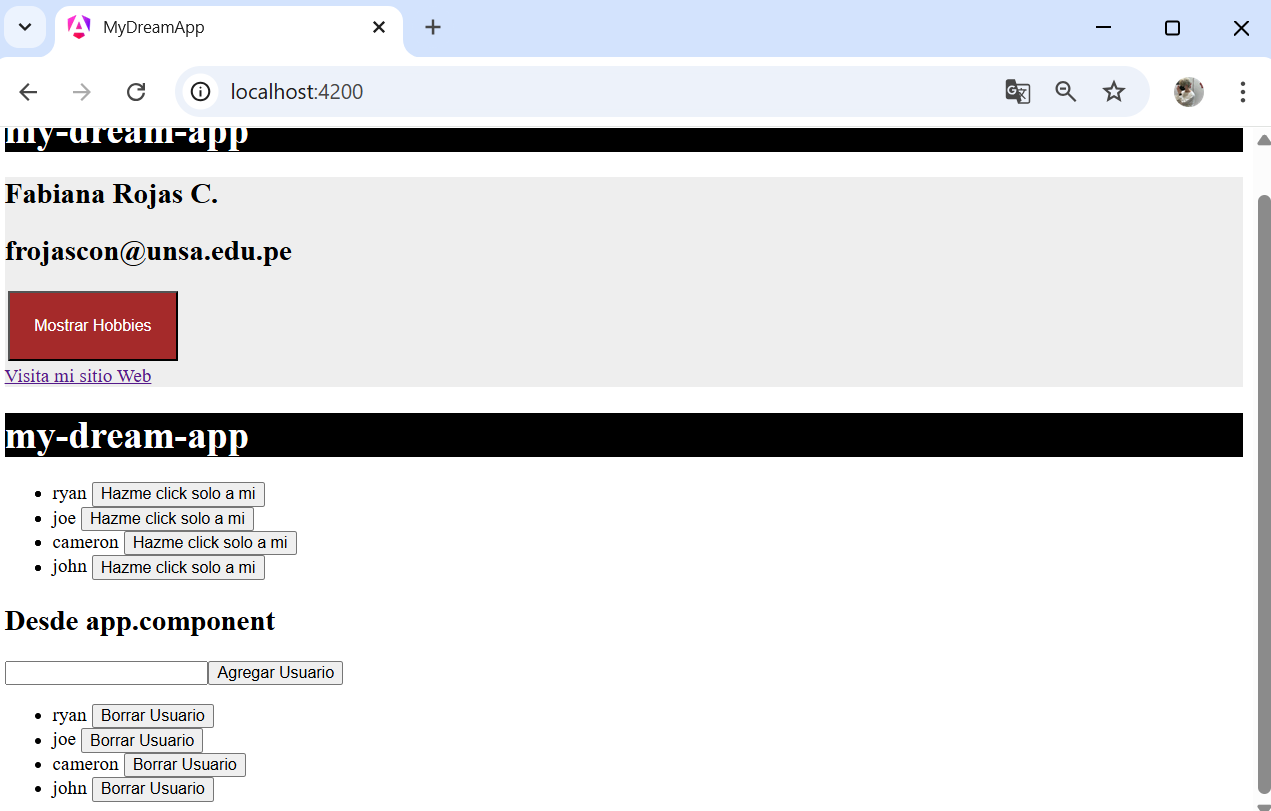
\includegraphics[width=1\textwidth,keepaspectratio]{imagenesInforme/P17.png}
		%\includesvg{imagenesInforme/P1.png}
		%\label{img:mot2}
		%\caption{Product backlog.}
	\end{figure}
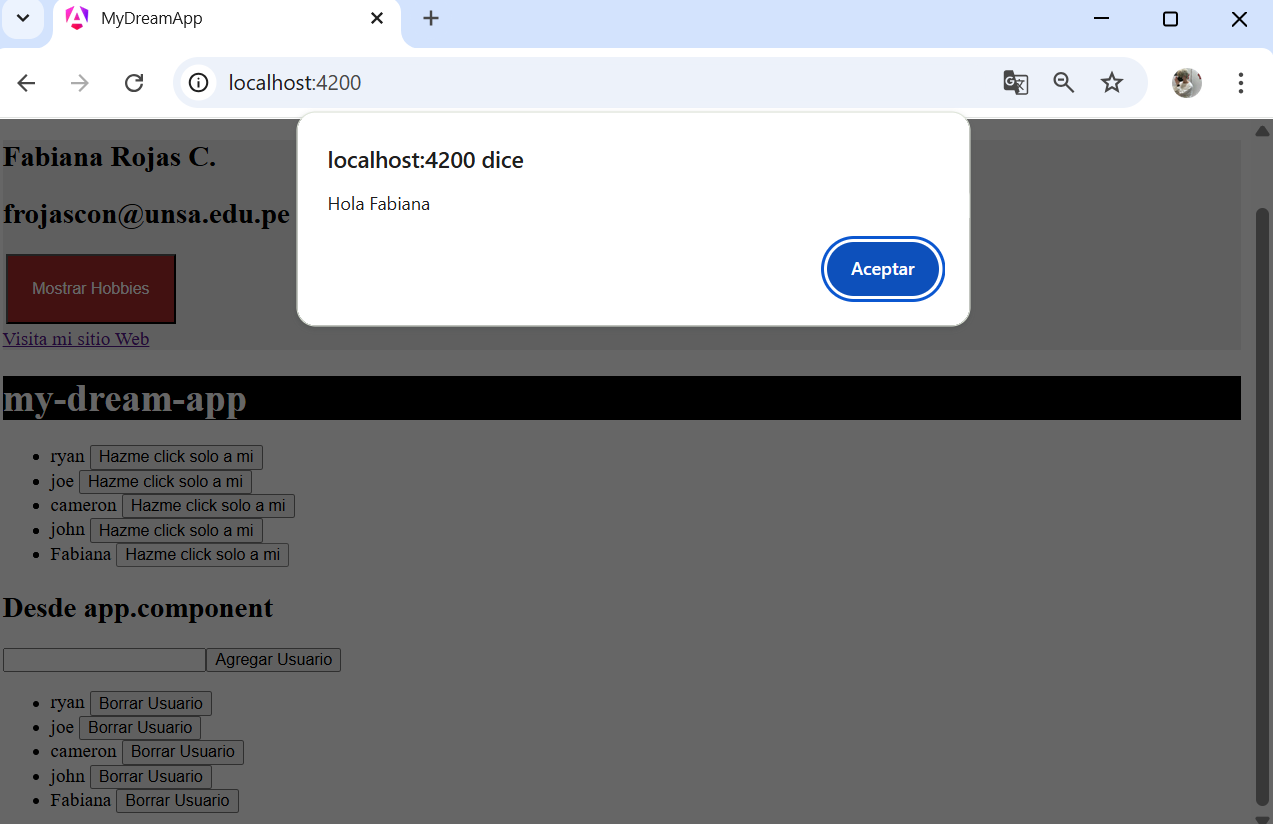
\includegraphics[width=1\textwidth,keepaspectratio]{imagenesInforme/P18.png}
		%\includesvg{imagenesInforme/P1.png}
		%\label{img:mot2}
		%\caption{Product backlog.}
	\end{figure}
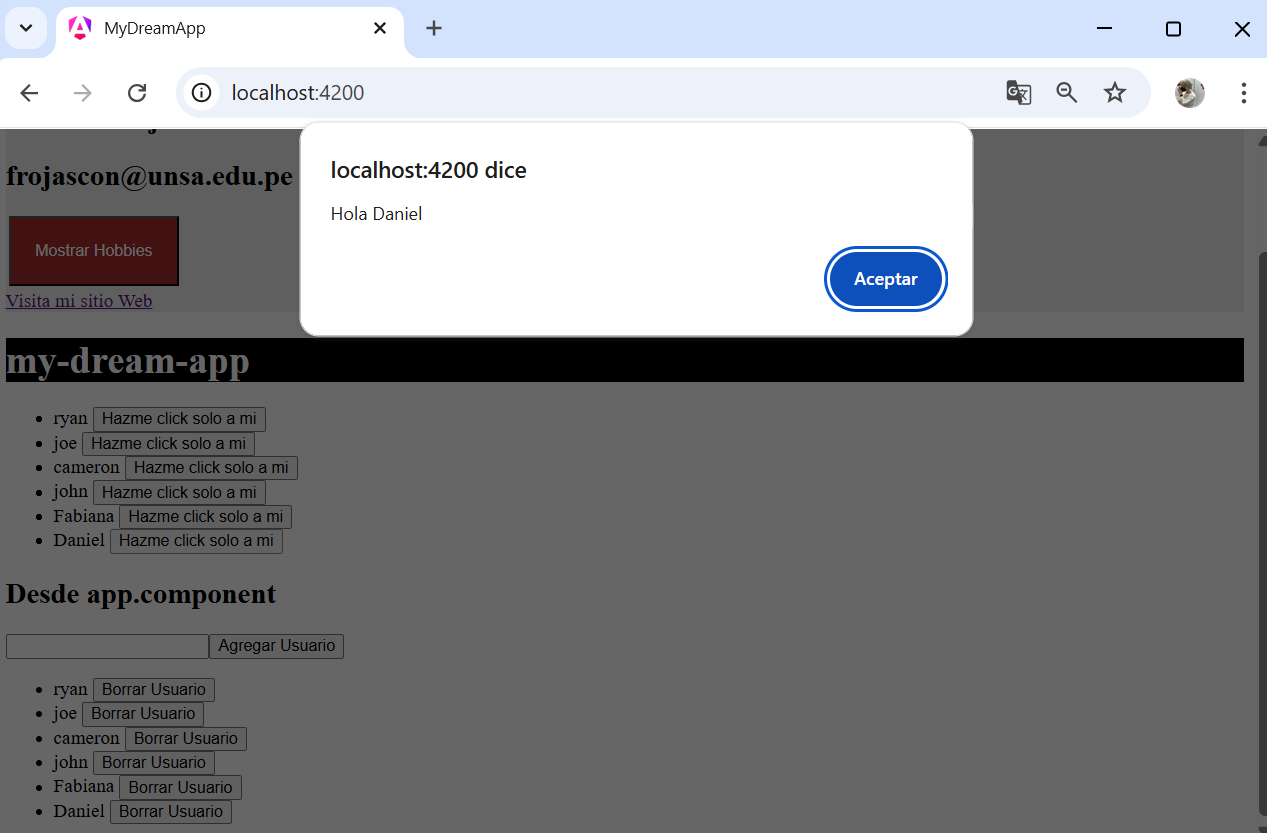
\includegraphics[width=1\textwidth,keepaspectratio]{imagenesInforme/P19.png}
		%\includesvg{imagenesInforme/P1.png}
		%\label{img:mot2}
		%\caption{Product backlog.}
	\end{figure}
\begin{lstlisting}
Commit 11:  "Angular2 - Diapositiva 4: Haciendo DataBinding con datos del formulario, se realizaron las indicaciones."
\end{lstlisting}
se implementó la funcionalidad de data binding utilizando el formulario para capturar y reflejar datos del usuario en tiempo real. Para ello, se incorporó FormsModule en el componente standalone y se utilizaron las directivas [(ngModel)] para enlazar los campos name y age con sus respectivas propiedades en la clase AppComponent. Al escribir en el formulario, los valores se actualizan automáticamente en la vista gracias a la vinculación bidireccional. 
\begin{center}
    \makebox[0pt]{Ejecución}
\end{center}
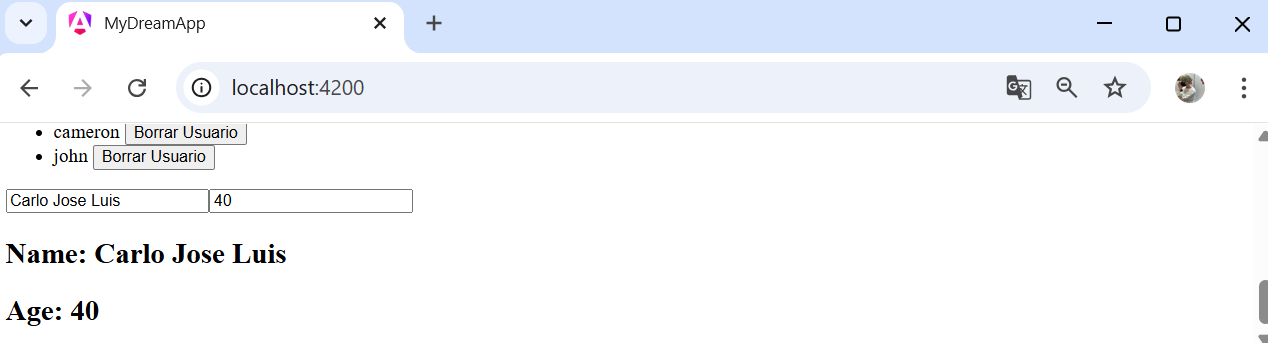
\includegraphics[width=1\textwidth,keepaspectratio]{imagenesInforme/P20.png}
		%\includesvg{imagenesInforme/P1.png}
		%\label{img:mot2}
		%\caption{Product backlog.}
	\end{figure}

\begin{lstlisting}
Commit 12: "Angular2 - Diapositiva 9,10,11: Insertando un Servicio para llamar a Json."
\end{lstlisting}
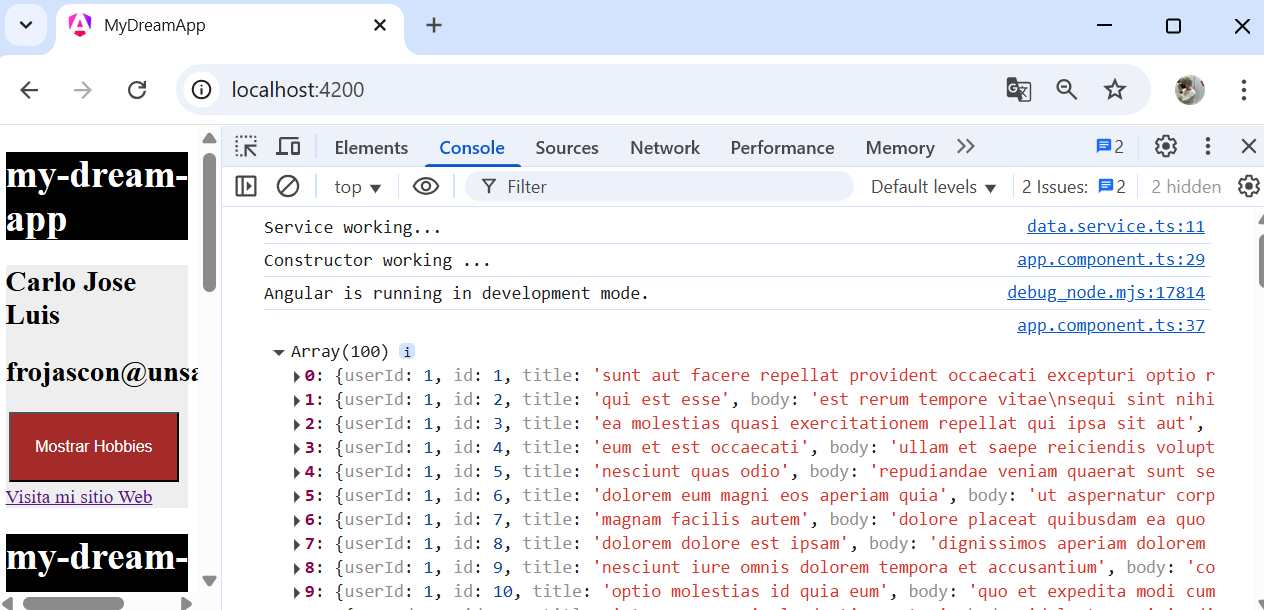
\includegraphics[width=1\textwidth,keepaspectratio]{imagenesInforme/P21.png}
		%\includesvg{imagenesInforme/P1.png}
		%\label{img:mot2}
		%\caption{Product backlog.}
	\end{figure}
\begin{lstlisting}
Commit 13: "Angular2 - Diapositiva 12: Insertando un Servicio para llamar a Json."
\end{lstlisting}
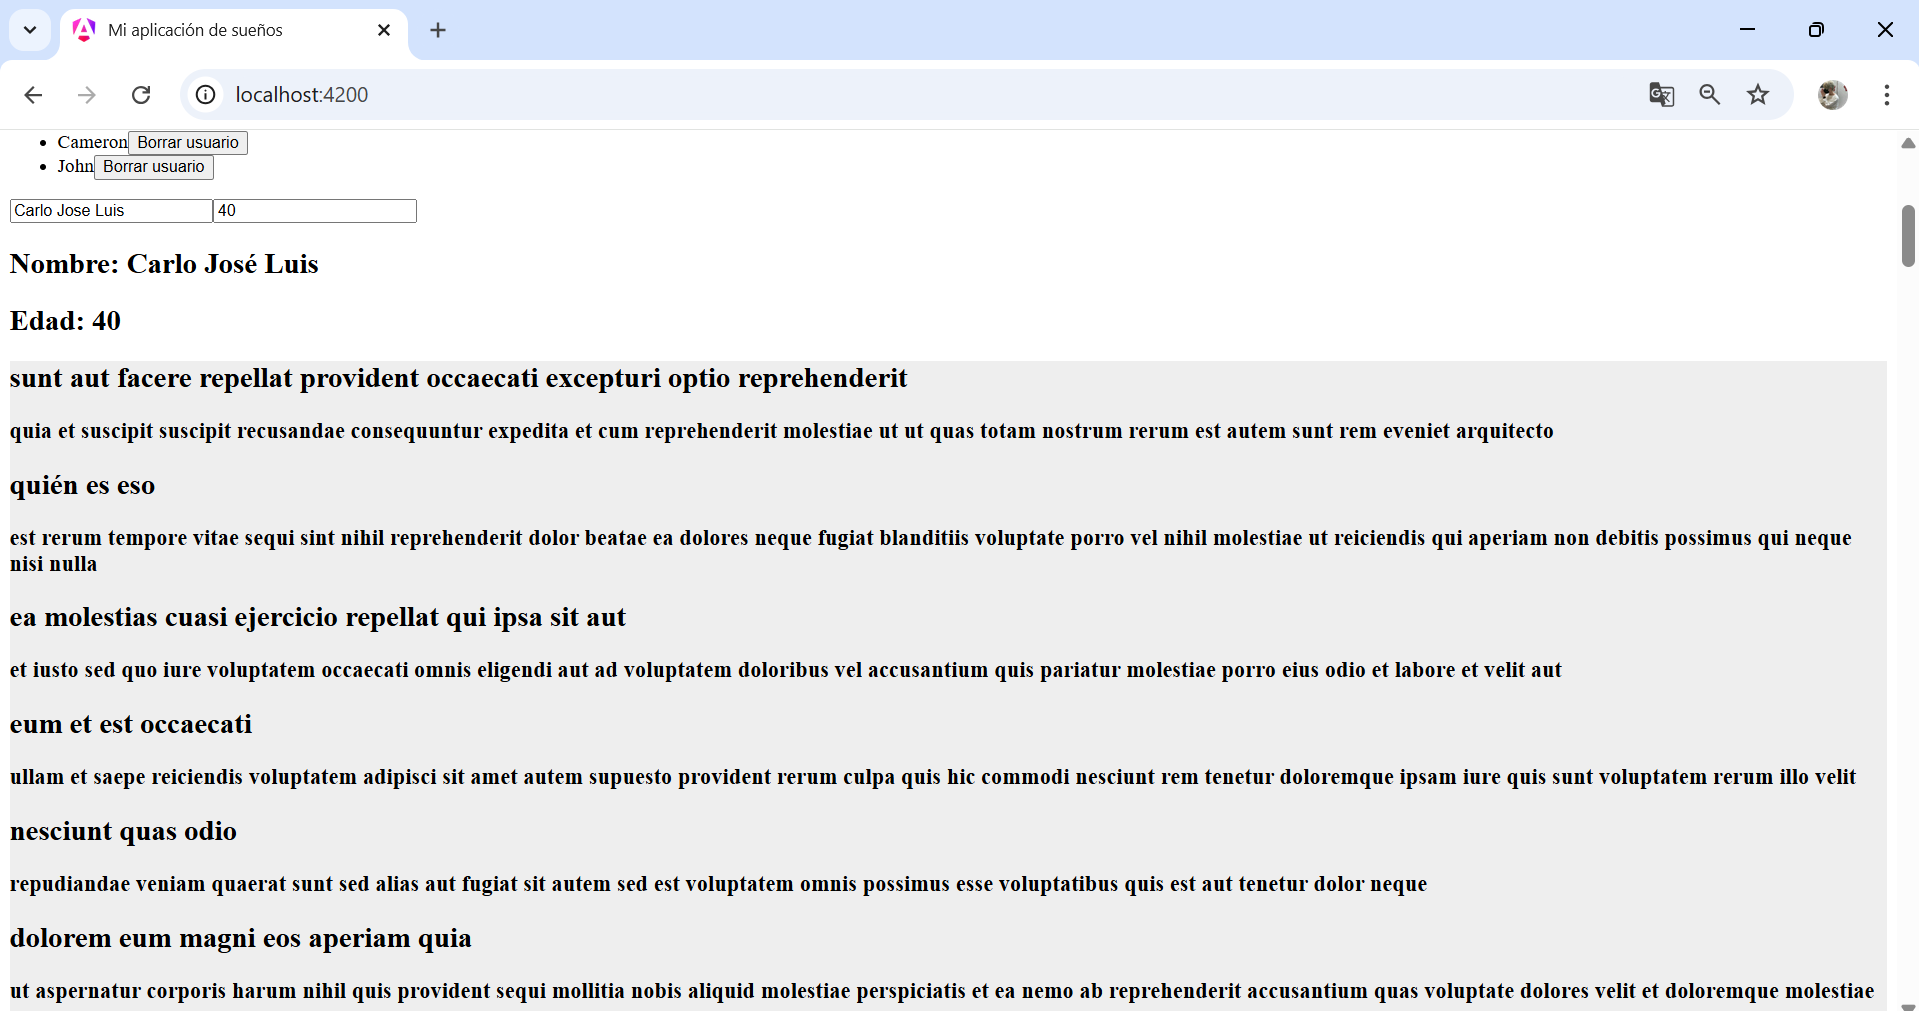
\includegraphics[width=1\textwidth,keepaspectratio]{imagenesInforme/P22.png}
		%\includesvg{imagenesInforme/P1.png}
		%\label{img:mot2}
		%\caption{Product backlog.}
	\end{figure}
\begin{lstlisting}
Commit 14: "Angular 2 - Diapositivas 15,16,17: Insertando Ruteos /about y /hello al proyecto para navegar a traves de la url"
\end{lstlisting}
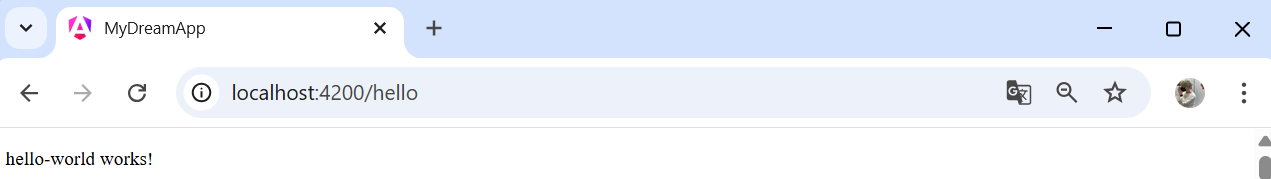
\includegraphics[width=1\textwidth,keepaspectratio]{imagenesInforme/P24.png}
		%\includesvg{imagenesInforme/P1.png}
		%\label{img:mot2}
		%\caption{Product backlog.}
	\end{figure}
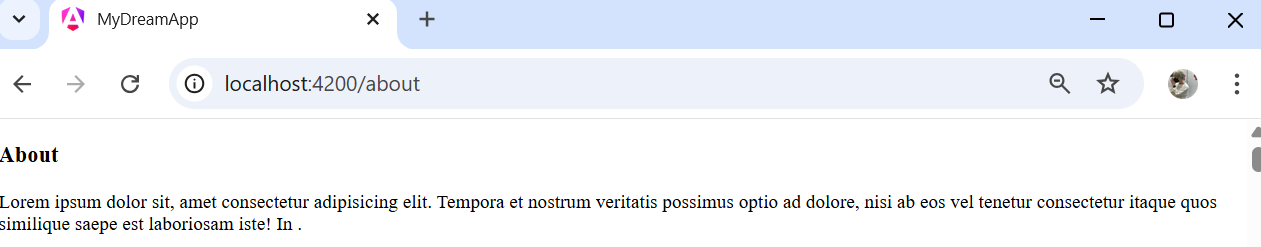
\includegraphics[width=1\textwidth,keepaspectratio]{imagenesInforme/P23.png}
		%\includesvg{imagenesInforme/P1.png}
		%\label{img:mot2}
		%\caption{Product backlog.}
	\end{figure}
\begin{lstlisting}
Commit 15: "Angular2 - Diapositiva 18: Se incorporo un menu para ruteos "
\end{lstlisting}
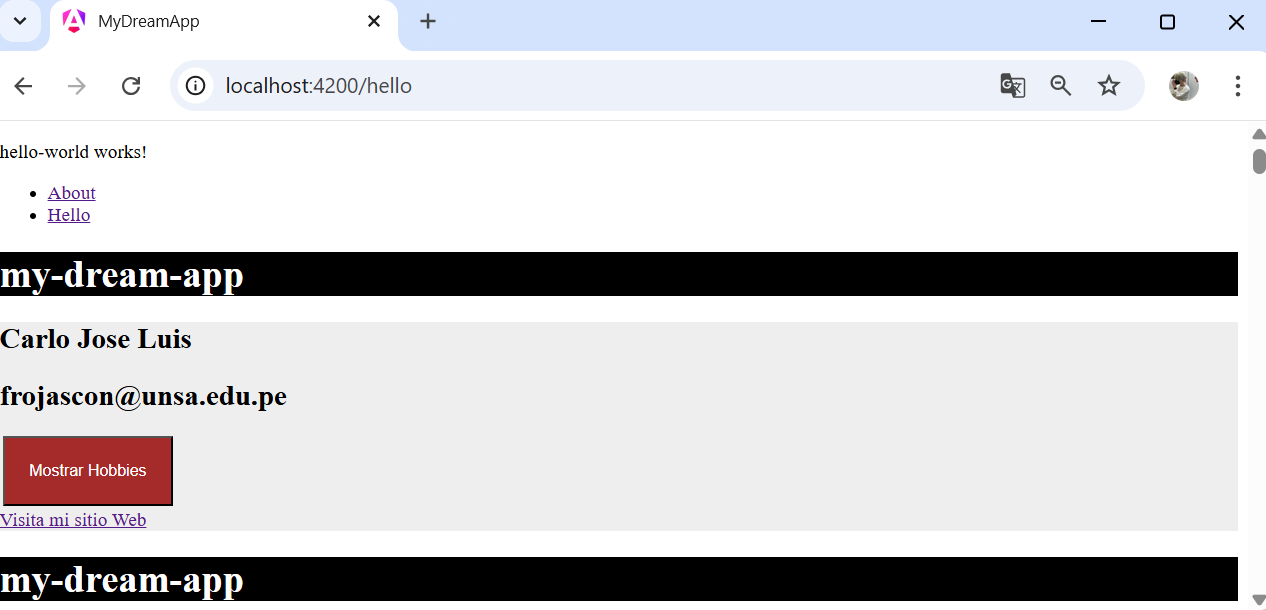
\includegraphics[width=1\textwidth,keepaspectratio]{imagenesInforme/P25.png}
		%\includesvg{imagenesInforme/P1.png}
		%\label{img:mot2}
		%\caption{Product backlog.}
	\end{figure}
			
	
			\section{Referencias}
			\begin{itemize}			
				\item \url{https://docs.google.com/presentation/d/1OaXlgzMSVr1M2mOqtqbT79x6ynWZjMdT/edit?slide=id.p1#slide=id.p1}
				\item \url{https://docs.google.com/presentation/d/1__PTJpPALSxu0leYlpGcqNKrzz4q2TZf/edit?slide=id.p1#slide=id.p1}
			\end{itemize}	
			
			%\clearpage
			%\bibliographystyle{apalike}
			%\bibliographystyle{IEEEtranN}
			%\bibliography{bibliography}
			
	     	\end{document}
